%% Tex spellcheck = fr_FR
\chapter{Chapter 5 : How GPS Coarse Acquisition Works}

This chapter will explain how the GPS \gls{ca} code works. How a single bit is received what's actually sent by the satellite, how the receiver correlates the received signal with the local replica of the signal, and how the receiver can determine the time of flight of the signal.


\section{Data Modulation}

When sending the actual data on the \textbf{L1} band, we're combining a carrier wave with the C/A code and the navigation data.

The navigation data actually contains:
\begin{itemize}
	\item The time at which the data was sent
	\item The \textbf{ephemeris} data, which is a set of data that describes the precise position of the satellite sending the data
	\item The \textbf{almanac}, which is a set of data that describes the coarse position of all the satellites in the constellation
	\item The satellite health/accuracy
	\item ionospheric model for correction
\end{itemize}

Here we can see how the data is modulated and sent.

\begin{figure}[H]
	\centering
	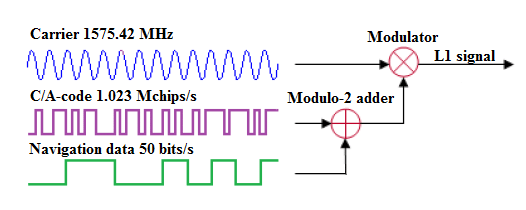
\includegraphics[width=1\linewidth]{modulation_nav_data.png}
	\caption[Navigaiton data modulation]{Navigaiton data modulation Source: www.e-education.psu.edu ref: URL14}
	\label{fig:nav_modulation}
\end{figure}



\section{Code Correlation}

As described in previous chapters, the GPS system uses a \gls{cdma} system to transmit the signals. This means that all the satellites are transmitting on the same frequency at the same time. The receiver needs to be able to distinguish the signal from each satellite. This is done by using a unique code for each satellite. The receiver knows the code of each satellite and can then correlate the received signal with the local replica of the signal. As described in the next figure, the correlation is done by multiplying the received signal with the local replica of the signal. The result of this multiplication is then integrated over a period of time. If the received signal is the same as the local replica, the correlation will be at its maximum. If the received signal is different, the correlation will be lower. This is how the receiver can distinguish the signal from each satellite.

\begin{figure}[H]
	\centering
	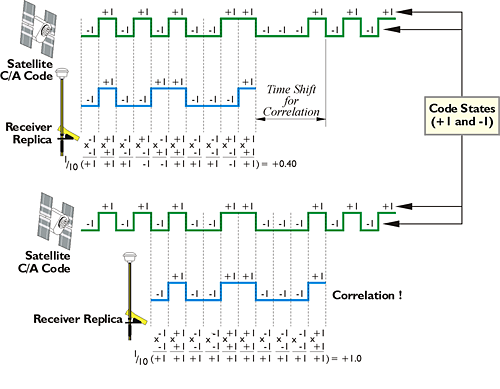
\includegraphics[width=1\linewidth]{correlation_prn.png}
	\caption[C/A PRN Correlation]{C/A PRN Correlation Source: www.e-education.psu.edu ref: URL14}
	\label{fig:prn_correlation}
\end{figure}


\section{Frame data}

The data sent by the satellite is divided into frames. Each frame contains 1500 bits and is sent at a rate of 50 bits per second. The frame is divided into 5 subframes, each divided into 10 words of 30 bits (300 bits per subframe). The full frame is sent every 30 seconds. The subframes one to three are sent fresh every frame but the subframes 4 and 5 contain the almanac data and are sent in multiple frames over time (25 frames for subframe 4 and 25 frames for subframe 5). The receiver can then reconstruct the full almanac data by combining the data from the different frames.


\begin{figure}[H]
	\centering
	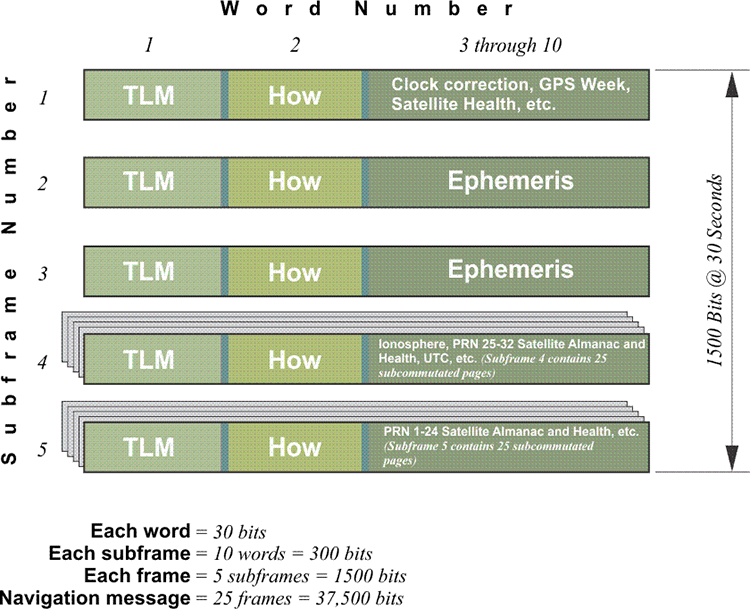
\includegraphics[width=1\linewidth]{nav_data.png}
	\caption[C/A PRN Correlation]{C/A PRN Correlation Source: www.e-education.psu.edu ref: URL15}
	\label{fig:nav_data}
\end{figure}

\section{Time and distance calculation}

We want to compute the distance between the satellite and the receiver. We know the speed of light and the time at which the signal was sent. We could compare it to the time at which the signal was received to get the time of flight of the signal to finally compute the distance, knowing the speed of light. However, this would mean that we have two absoulutely precise and perfectly synchronized oscillators in the receiver and the satellite.

It would be kind of impossible nor would it be economically viable to have atomic clocks in every receiver devices. This is why the \gls{gps} actually uses the position and time of four satellites to solve a four equations system to determine the position of the receiver. This is called \textbf{differential positioning}.


\begin{figure}[H]
	\centering
	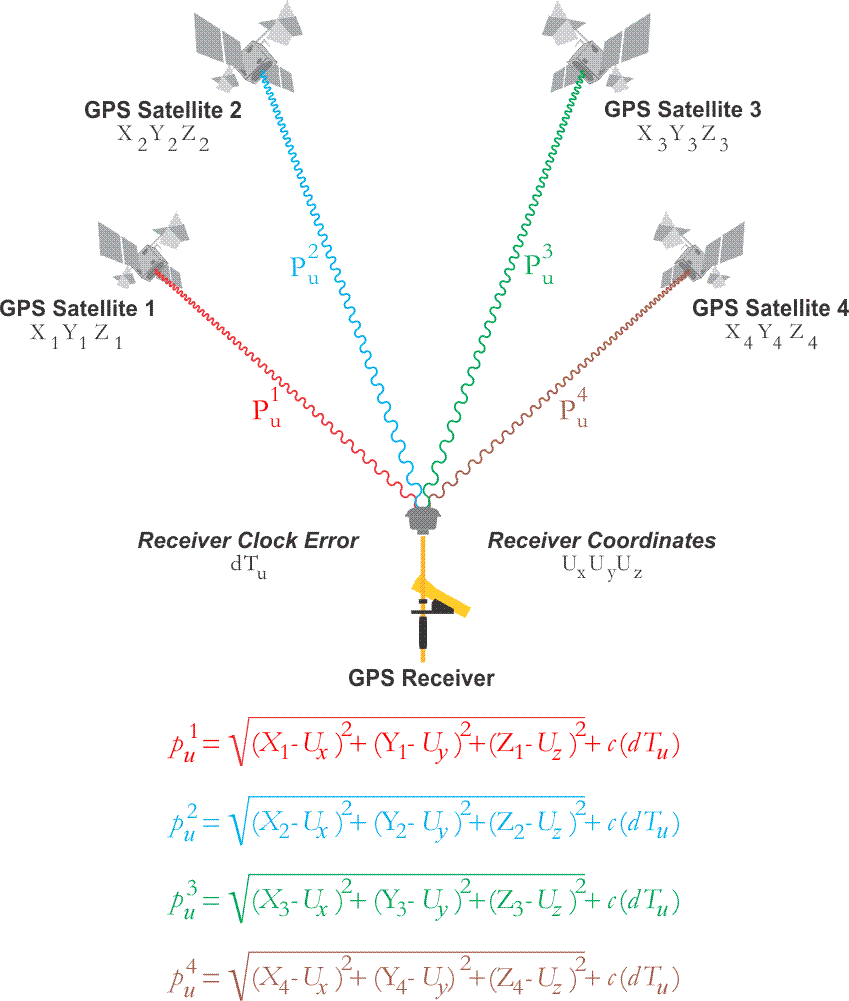
\includegraphics[width=0.8\linewidth]{differential_position.png}
	\caption[Differential positionning equations]{Differential positionning equations Source: www.e-education.psu.edu ref: URL16}
	\label{fig:differential_position}
\end{figure}





